\documentclass[tikz,border=10pt]{standalone}
\usepackage{pgfplots}
\pgfplotsset{compat=1.18}
\usepgfplotslibrary{colorbrewer}

\begin{document}
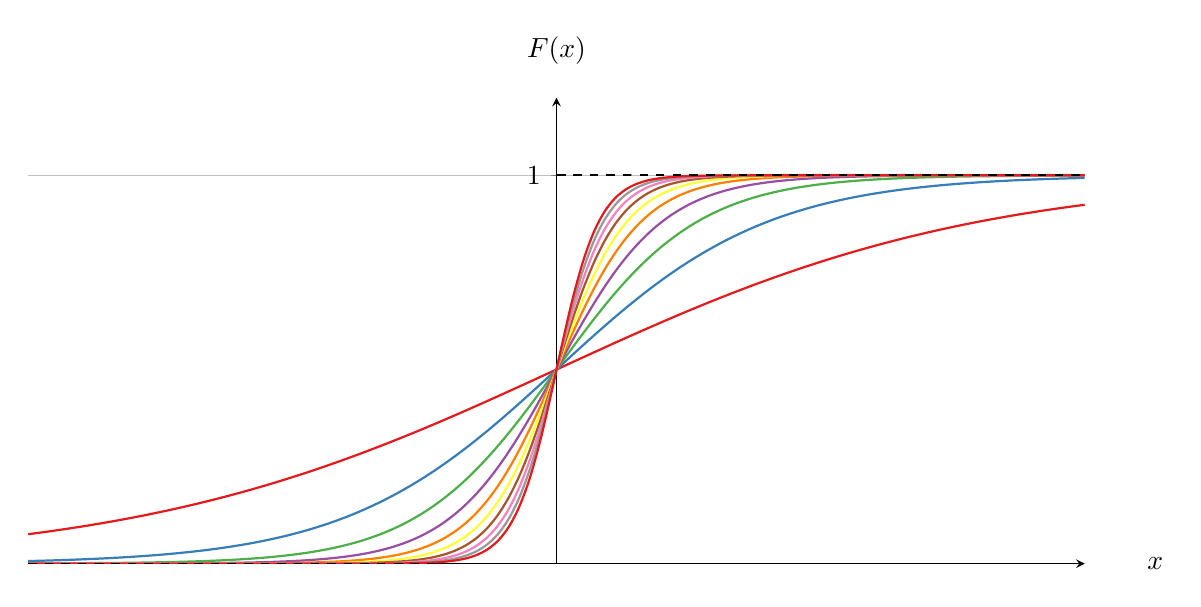
\begin{tikzpicture}
\begin{axis}[
    axis lines=middle,
    width=15cm, height=7.5cm,  % Adjusting the aspect ratio
    xmin=-5, xmax=5,
    ymin=0, ymax=1.2,
    xlabel=$x$,
    ylabel=$F(x)$,
    every axis x label/.style={
        at={(ticklabel* cs:1.05)},
        anchor=west,
    },
    every axis y label/.style={
        at={(ticklabel* cs:1.05)},
        anchor=south,
    },
    xtick={0},
    ytick={0,1},
    xticklabels={$0$},
    yticklabels={$0$, $1$},
    samples=100,
    grid=both,
    grid style={line width=.1pt, draw=gray!10},
    major grid style={line width=.2pt,draw=gray!50},
    cycle list/Set1-9,
    legend style={draw=none}, % This disables the legend border
    % legend entries={},        % This sets the legend entries to empty
]

% Plotting more logistic curves with colors
\foreach \a in {0.5,1,...,5} {
    \addplot+ [domain=-5:5, smooth, thick] {1/(1+exp(-\a*x))};
}

% Plotting the piecewise function
\addplot [domain=-5:0, smooth, thick, dashed, black] {0};
\addplot [domain=0:5, smooth, thick, dashed, black] {1};

\end{axis}
\end{tikzpicture}
\end{document}
